\section{Experimental Setup}
\label{sec:experiment}

We use a commercial tool set Xtensa RD-2011.2 from Tensilica Inc., \ref{}. Our base processor is Xtensa LX2 extensible cores and its configurations are summarized in Table \ref{tab:p_config}. The tool set includes C/C++ compiler that can compile C/C++ code for the target LX2 processor. The target application is simulated in the Instruction Set Simulator (ISS) that is included in the toolset. We use the Xtensa PRocessor Extension Synthesis (XPRES) compiler provided by the toolset to generate the various customized versions of the tasks. The newly generated task versions consist of any combination of fused operations, FLIX instructions, vector operations and specialized operations. 
%Figure \ref{} shows the performance vs area trade off for various customized versions of the tasks. 

In our experiments, we use five different instruction cache configurations ranging from 1 KB to 16 KB. Table \ref{tab:p_config} shows the area consumed by various cache configurations. We modify only instruction cache, but our technique can easily be extended to data cache too. We use Xt-Xenergy tool included in the toolset to measure both the dynamic and leakage energy consumptions. We use five different frequency levels ranging from 1.5 Ghz to 533 Mhz. We always set the voltage that supports the frequency being set ~\ref{}. We perform all our simulations at the maximum frequency and voltage. We estimate the power consumption at the frequency level $i$ using the following equation,
\begin{equation}
P_i = \frac{P_{max} * (V_i)^2 * F_i} {(V_{max})^2 * F_{max}}
\end{equation}  

We use popular streaming applications like MP3 encoder and JPEG encoder. Figure \ref{fig:benchmark} shows the various compute intensive kernels in the application. 

\begin{figure}[h]
\label{fig:benchmark}
\center
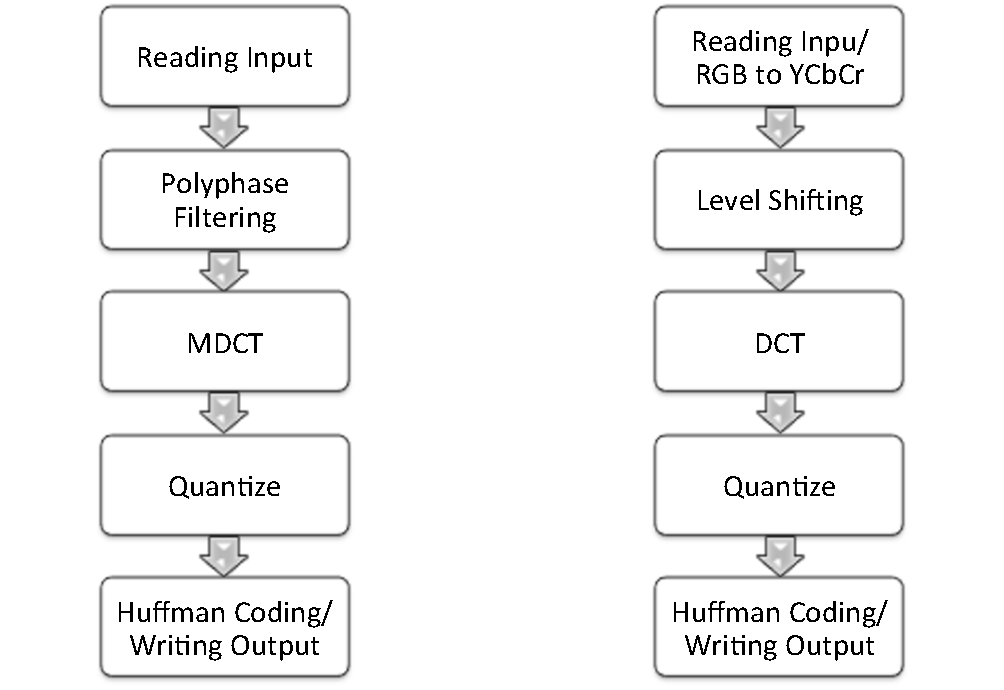
\includegraphics[width=0.40\textwidth, height=0.32\textwidth]{benchmark.pdf}
\label{fig:cache-size}
\caption {MP3 and JPEG}
\end{figure}

\begin{center}
\begin{table}
\begin{tabular}{|c|c|}
\hline
Frequency & 1.5 Ghz\ \\
\hline
Pipeline Depth & 5\ \\
\hline
Process Techology & 65nm GP \ \\
\hline
Core Area & 82806 gates or 0.451 $mm^2$\ \\
\hline
Max Instruction Width & 8 bytes\ \\
\hline
Data Cache size & 32 KB\ \\
\hline
Instruction Cache Size & 0.452 $mm^2$,\ \\
16K, 8K, 4K, 2K, 1K  & 0.275 $mm^2$, 0.174 $mm^2$,\ \\
 & 0.124 $mm^2$, 0.103 $mm^2$\ \\
\hline
I-Cache \& D-cache line size & 16 bytes\ \\
\hline
I-Cache \& D-cache Assoc & Direct mapped\ \\
\hline
PIF Interface & 32 bytes\ \\
\hline
Other Features & Boolean Registers, MUL32 \ \\ 
& and MAC16 instructions\ \\
& Functional unit clock gating,\ \\ 
& Flip-Flop register files\ \\
\hline
\end{tabular}
\caption{Baseline Processor Configuration.}
\label{tab:p_config}
\end{table}
\end{center}